\documentclass[aspectratio=169,
hyperref={colorlinks,urlcolor=blue}
]{beamer}

%\usetheme{Pittsburgh}
\usetheme{default}
\usepackage{colortbl}%colored tables
%For using helvetica font:
\usepackage[scaled]{helvet}
\usepackage[T1]{fontenc}
\renewcommand\familydefault{\sfdefault}
\urlstyle{same} %sets the fonts for urls
\usepackage{pdfpages}
\usepackage{siunitx}
\usepackage{caption}
\usepackage{pifont}%for dings
\usepackage{pgfplots}%for 3d plotting
\pgfplotsset{compat = newest}
\usepackage{mathtools}%box in align env \Aboxed
\usepackage[american,smartlabels]{circuitikz}%for drawing circuits
\usepackage{multimedia}
\usepackage{animate}
\usepackage{xcolor}


\usetikzlibrary{arrows}
\usetikzlibrary {3d} 
\usetikzlibrary{decorations.markings, math}
\usetikzlibrary{intersections, pgfplots.fillbetween}
\usetikzlibrary {shapes.geometric} 


%\definecolor{myblue}{RGB}{5, 34, 150}
\definecolor{myblue2}{RGB}{5, 34, 150}
\definecolor{myblue}{RGB}{0,36,82}
\definecolor{myred}{RGB}{207, 2, 13}
\definecolor{mygreen}{RGB}{0, 158, 11}
\definecolor{myyellow}{RGB}{220,220,0}
\definecolor{qblue}{RGB}{0,36,82}
\definecolor{qgold}{RGB}{250,189,15}
\definecolor{qred}{RGB}{185,14,49}
\definecolor{cblue}{rgb}{0.13, 0.67, 0.8}
\definecolor{corange}{rgb}{0.8, 0.34, 0.0}
\definecolor{cpurple}{rgb}{0.54, 0.29, 0.42}

%%%%%%%%%%%% General settings
\setbeamercolor{frametitle}{fg=black}
\setbeamercolor{title}{fg=black}
\setbeamercolor{author}{fg=myblue2}

\beamertemplatenavigationsymbolsempty %no navigation controls at bottom of slides
%\setbeamertemplate{footline}[frame number]
\usefonttheme{professionalfonts} 
\setbeamerfont{title}{series=\bfseries,parent=structure}
\setbeamerfont{frametitle}{series=\bfseries,parent=structure}

%%%%%%%%%%%%Lists
\setbeamertemplate{itemize item}[circle] %{\color{myblue}$\circ$}
\setbeamertemplate{itemize subitem}{\color{myblue2}$\circ$}
\setbeamertemplate{itemize subsubitem}{\color{myblue2}$\cdot$}
\setbeamercolor{itemize item}{bg=myblue2,fg=myblue2}
\setbeamercolor{enumerate item}{bg=myblue2,fg=myblue2}
%%%%%%%%%%%%%%%%%%%%%%%%%%%%

%%%%%%%%%%%%Blocks
\setbeamertemplate{blocks}[rounded]
%Default block
\setbeamercolor{block title}{bg=myblue2, fg=white}
\setbeamercolor{block body}{bg=myblue2!10}
\setbeamerfont{block body}{size=\scriptsize}
\setbeamerfont{block title}{size=\scriptsize}
%Alert block
\setbeamercolor{block title alerted}{bg= myblue2, fg=white}
\setbeamercolor{block body alerted}{bg=myblue2!10}
\setbeamerfont{block body alerted}{size=\scriptsize}
\setbeamerfont{block title alerted}{size=\scriptsize}
%example block
\setbeamercolor{block title example}{bg=mygreen, fg=white}
\setbeamercolor{block body example}{bg=mygreen!10}
\setbeamerfont{block body example}{size=\scriptsize}
\setbeamerfont{block title example}{size=\scriptsize}
%%%%%%%%%%%%%%%%55


%%%%%%%%%%%%Figures and captions
\captionsetup{font=scriptsize,labelfont=scriptsize}
%\setbeamertemplate{caption}{\raggedright\insertcaption\par}
\newenvironment{capfig}[3]{\begin{figure}\includegraphics[width=#1\textwidth]{#2}\caption*{\textit{#3}}\end{figure}}{}

%\makeatother
%\setbeamertemplate{footline}
%{
%  \leavevmode%
%  \hbox{%
%  \begin{beamercolorbox}[wd=.4\paperwidth,ht=2.25ex,dp=1ex,center]{author in head/foot}%
%    \usebeamerfont{author in head/foot}\insertshortauthor
%  \end{beamercolorbox}%
%  \begin{beamercolorbox}[wd=.6\paperwidth,ht=2.25ex,dp=1ex,center]{title in head/foot}%
%    \usebeamerfont{title in head/foot}\insertshorttitle\hspace*{3em}
%    \insertframenumber{} / \inserttotalframenumber\hspace*{1ex}
%  \end{beamercolorbox}
%  }%
%  \vskip0pt%
%}
%\makeatletter

\makeatother
\setbeamertemplate{footline}
{
  \leavevmode%
  \hbox{%
\begin{beamercolorbox}[wd=.27\paperwidth,ht=2.25ex,dp=1ex,center]{author in head/foot}%
    \color{black}{\insertinstitute}
\end{beamercolorbox}
  \begin{beamercolorbox}[wd=.27\paperwidth,ht=2.25ex,dp=1ex,center]{author in head/foot}%
    \color{black}{\inserttitle}
  \end{beamercolorbox}%
  \begin{beamercolorbox}[wd=.27\paperwidth,ht=2.25ex,dp=1ex,center]{title in head/foot}%
    \color{black}{\insertshortauthor}
  \end{beamercolorbox}
  \begin{beamercolorbox}[wd=.27\paperwidth,ht=2.25ex,dp=1ex,center]{title in head/foot}%
    \hspace{.28\paperwidth}\color{black} \insertframenumber{} / \inserttotalframenumber\hspace*{1ex}
  \end{beamercolorbox}
  }%
  \vskip0pt%
}
\makeatletter

\setbeamertemplate{title page}
{
  \begin{tikzpicture}[remember picture,overlay]
    \def\barh{4}%15
  
    \draw[color=myblue2,line width=\barh] ([yshift=-0.5*\barh]current page.north west) -- ([yshift=-0.5*\barh,xshift=-0.67\paperwidth]current page.north east);
    \draw[color=myblue2,line width=\barh] ([yshift=-0.5*\barh,xshift=-0.67\paperwidth]current page.north east) -- ([yshift=-0.5*\barh,xshift=-0.34\paperwidth]current page.north east);
    \draw[color=myblue2,line width=\barh] ([yshift=-0.5*\barh,xshift=-0.34\paperwidth]current page.north east) -- ([yshift=-0.5*\barh]current page.north east); 
  
    \draw[color=myblue2,line width=\barh] ([yshift=0.5*\barh]current page.south west) -- ([yshift=0.5*\barh,xshift=-0.67\paperwidth]current page.south east);
    \draw[color=myblue2,line width=\barh] ([yshift=0.5*\barh,xshift=-0.67\paperwidth]current page.south east) -- ([yshift=0.5*\barh,xshift=-0.34\paperwidth]current page.south east);
    \draw[color=myblue2,line width=\barh] ([yshift=0.5*\barh,xshift=-0.34\paperwidth]current page.south east) -- ([yshift=0.5*\barh]current page.south east);
    %\node[left] at (current page.east) {
    %
\includegraphics[scale=0.1]{figures/coverpage}
    %};
  \end{tikzpicture}
  
  \usebeamerfont{title}\usebeamercolor[fg]{title}\inserttitle\par
  \usebeamerfont{subtitle}\usebeamercolor[fg]{subtitle}\insertsubtitle\par
  \vspace{2cm}
  \usebeamerfont{author}\usebeamercolor[fg]{author}\insertauthor\par
  \usebeamerfont{institute}\usebeamercolor[fg]{author}\insertinstitute\par
  \usebeamercolor[fg]{author}\par
  \usebeamercolor[fg]{titlegraphic}\inserttitlegraphic

} 

\setbeamertemplate{frametitle}{%
    \nointerlineskip%
        \par\hspace*{-\dimexpr0.5\paperwidth-0.5\textwidth}\textcolor{myblue2}{\rule{0.33\paperwidth}{6pt}}\textcolor{myblue2}{\rule{0.33\paperwidth}{6pt}}\textcolor{myblue2}{\rule{0.34\paperwidth}{6pt}} 
    \begin{beamercolorbox}[wd=\paperwidth,ht=0.75cm,dp=0.6ex]{frametitle}
        \hspace*{0.5cm}\strut\usebeamerfont{frametitle}\insertframetitle\strut
        %\hrule
    \end{beamercolorbox}%
    %%Line below:
%\par\hspace*{-\dimexpr0.5\paperwidth-0.5\textwidth}\textcolor{myblue}{\rule{\paperwidth}{0.4pt}}
     % <-- calculation of left margin width + rule
     %\textcolor{red}{\noindent\rule{\paperwidth}{2pt}}
}


%%%%%%%%%%%%Frame templates

%Slide with title
\newenvironment{titleframe}[1]
{\begin{frame}\frametitle{#1}\end{frame}}
{}

%Slide with title and itemize list:
\newenvironment{bulletframe}[1]
{\begin{frame}{#1} \itemize}
{\enditemize \end{frame}}

%Slide with two columns 50/50
\newenvironment{twocolframe}[3]
{\begin{frame}{#1}
 \begin{columns}[T]
 \column{0.5\textwidth}#2
 \column{0.5\textwidth}#3
 \end{columns}\end{frame}}{}

%Slide with two columns 60/40 <<<<<<<<<<<<<<<<<<<<<<  This one!
\newenvironment{twocolframesf}[3]
{\begin{frame}{#1}
 \begin{columns}[T]
 \column{0.6\textwidth}#2
 \column{0.4\textwidth}#3
 \end{columns}\end{frame}}{}
 
%Slide with two columns 70/30
\newenvironment{twocolframest}[3]
{\begin{frame}{#1}
 \begin{columns}[T] 
 \column{0.7\textwidth}#2
 \column{0.3\textwidth}#3
 \end{columns}\end{frame}}{} 
 
%Slide with two columns 40/60
\newenvironment{twocolframefs}[3]
{\begin{frame}{#1}
 \begin{columns}[T] 
 \column{0.4\textwidth}#2
 \column{0.6\textwidth}#3
 \end{columns}\end{frame}}{}
 
%Slide with two columns 70/30
\newenvironment{twocolframets}[3]
{\begin{frame}{#1}
 \begin{columns}[T] 
 \column{0.3\textwidth}#2
 \column{0.7\textwidth}#3
 \end{columns}\end{frame}}{} 

 
%Colloquium speaker (title, abstract, picture file, speaker name)
\newenvironment{colloquium}[5]
{
\begin{frame}{Colloquium: Friday 1:30pm in Stirling A}
\begin{columns}[T] 
 \column{0.8\textwidth}
 \textbf{#1}\\
 #2
 \column{0.2\textwidth}
 \capfig{#3}{#4}{#5}
 \end{columns}
\end{frame}
}
{} 

%%%%%%%%%%%%%Set Hyperref colors


\hypersetup{
  colorlinks=true,
  linkcolor=blue,    
  urlcolor=blue,     
  citecolor=blue      
}
%%%%%%%%%%%%%TOC bolding
\setbeamerfont{section in toc}{series=\bfseries}



%Frames:
% \twocolframesf 60/40 (fs, st, ts) 
% \titleframe
% bulletframe


%%%%%%%%%%%%%%%%%%%%%%%%%
%%%%%% START OF PRESENTATION %%%%%%
%%%%%%%%%%%%%%%%%%%%%%%%%
\title{Gauss}
\subject{Gauss's Law, Flux and Application}
\subtitle{Building Models to Describe our World}


%%%%%%%%%%%%%%%%%%%%%%%%%%%%%%
%%%%%%%%%%%%%%%%%%%%%



\begin{document}

%%%%%%%%%%%%%%%%%%%%%%%%%
%%%%%% Title slide %%%%%%
%%%%%%%%%%%%%%%%%%%%%%%%%
\chaptertitle{Gauss}
\begin{frame}
\titlepage
\thispagestyle{empty}

\begin{textblock*}{5cm}(11cm,4cm)
    
\includegraphics[width=4cm]{figures/BMDW/logo}
\end{textblock*}

\end{frame}

%%%%%%%%%%%%%TOC
\twocolframe{Outline}
  {\tableofcontents[sections={1}, subsectionstyle=show/show]\thispagestyle{empty}}
  {\tableofcontents[sections={2,3}, subsectionstyle=show/show]}
%%%%%%%%%%%%%%%%%%%%%%%%%



\section{Gauss's Law and Flux}
\label{sec:gausssslawandflux}
\title{Gauss's Law and Flux}


%%%%%%%%%%%%%%%%%%%%%%%%%
\begin{frame}
\titlepage
\thispagestyle{empty}
\end{frame}

%



\subsection{Formula}
\label{subsec:formula}
\begin{frame}{Gauss's Law}
\begin{align*}
\Aboxed{\Phi_E &= \frac{Q^{enc}}{\epsilon_0}}
\end{align*}
\end{frame}



%%%%%%%%%%%%%%%%%%%%%%%%%%%%%%%%
\subsection{What is "flux"?}
\label{subsec:whatisflux}
\begin{frame}{An analogy to understand flux through a closed surface}

\begin{center}

\begin{animateinline}[autoplay,loop]{5} % 5 fps, same as 0.2 s transduration

\multiframe{20}{i=0+1}{

\begin{tikzpicture}
\tikzmath{
\R=0.5;
\r=0.6+0.1*\i;
}
\useasboundingbox (-3,-2.5) rectangle (3,2.5);

\scalebox{1}{

\fill[color=myred] (0,0) circle(\R);
\foreach \th in{0,30,...,330}{
  \fill[color=myblue!60] (\th:\r) circle(2pt);
}

}
\end{tikzpicture}

}
\end{animateinline}
\captionof*{figure}{\textit{Pellets being emitted isotropically by a source.}}
\end{center}


 \begin{itemize}
 \item A ``source'' emits little pellets isotropically (with spherical symmetry).
 \item Every second, the source emits 12 pellets.
 \end{itemize}
\end{frame}


%%%%%%%%%%%%%%%%%%%%%%%%%%%%%%%%



%%%%%%%%%%%%%%%%%%%%%%%%%%%%%%%%
\begin{frame}{An analogy to understand flux through a closed surface}

 \begin{itemize}
 \item One can think of flux as the number of pellets that are coming out of the source and crossing the closed surface.
 \item The flux through the closed surface does not depend on the surface, it only depends on the source!
 \end{itemize}
 

\begin{center}

\begin{animateinline}[autoplay,loop]{5} % 5 fps, same as 0.2 s transduration

\multiframe{20}{i=0+1}{

\begin{tikzpicture}
\tikzmath{
\R=0.5;
\r=0.6+0.1*\i;
}
\useasboundingbox (-6,-2.5) rectangle (6,2.5);

\scalebox{1}{

\begin{scope}[shift={(-3,0)}]
\fill[color=myred] (0,0) circle(\R);
\foreach \th in{0,30,...,330}{
  \fill[color=myblue!60] (\th:\r) circle(2pt);
}
\draw[line width=2] circle (1.5);
\end{scope}

\begin{scope}[shift={(3,0)}]
\fill[color=myred] (0,0) circle(\R);
\foreach \th in{0,30,...,330}{
  \fill[color=myblue!60] (\th:\r) circle(2pt);
}
\draw[line width=2] plot[smooth] coordinates{(0:1.25) (30:0.75) (60:1) (90:0.75) (135:1.5) (180:2.2) (225:1.5) (270:0.75) (300:1) (0:1.25)};
\end{scope}

}
\end{tikzpicture}

}
\end{animateinline}
\captionof*{figure}{\textit{Pellets being emitted isotropically by a source.}}
\end{center} 
 
\end{frame}


%%%%%%%%%%%%%%%%%%%%%%%%%%%%%%%%



%%%%%%%%%%%%%%%%%%%%%%%%%%%%%%%%
\subsection{Flux with distance}
\label{subsec:fluxwithdistance}
\begin{frame}{$1/R^2$}
\begin{itemize}
  \item The flux of pellets per unit area through a spherical surface decreases as:
  \begin{align*}
  N(R)\propto \frac{1}{4\pi R^2}
  \end{align*}
  \item This gives us a sense of how the electric force (or any $1/R^2$ force) is actually transmitted:
  \begin{itemize}
    \item Rather than action at a distance, maybe it’s more like particles being emitted from a charge and the force being related to the density of particles that is being felt (the particles are photons for the electric force).
  \item We had already argued that waves also have intensities that decrease as $1/R^2$, so maybe waves transmit these forces (light waves transmit the electric force)
  \item Wait, what? (photons are particles of light and light waves, it’s weird!)
  \item[$\rightarrow$] Gravity waves (confirmed), gravitons (particles for gravity, one of the major problems in physics!)

  \end{itemize} 

\end{itemize} 
\end{frame}

%%%%%%%%%%%%%%%%%%%%%%%%%%%



\subsection{Gauss's Law}
\label{subsec:gaussslaw}
\twocolframesf{Gauss' Law}
{ 
\begin{align*}
\Phi_E=\frac{Q^{enc}}{\epsilon_0}
\end{align*}
\begin{itemize}
 \item The flux of a field (e.g. Electric Field) across a \textbf{closed surface} only depends on the source (e.g. Charge) enclosed by that surface.
 \item Think of flux through a surface as the total number of ``pellets' hitting the surface or the number of field lines crossing the surface.
 \end{itemize}
}
{
\begin{center}
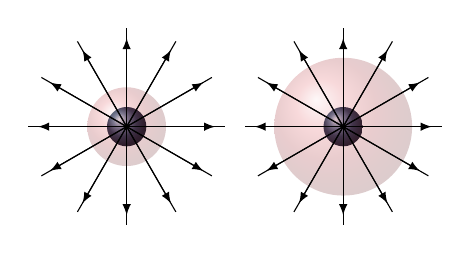
\begin{tikzpicture}
\tikzmath{
\R=0.25;
}
\scalebox{1}{

\shade[ball color=myblue!80] (0,0) circle(\R);
\shade[ball color=myred, opacity=0.2] (0,0) circle(2*\R);
\foreach \th in {0,30,...,330}{
\draw (0,0) -- (\th:5*\R);
\draw[-latex] (0,0) -- (\th:4.5*\R);
}

\begin{scope}[shift={(11*\R,0)}]

\shade[ball color=myblue!80] (0,0) circle(\R);
\shade[ball color=myred, opacity=0.2] (0,0) circle(3.5*\R);
\foreach \th in {0,30,...,330}{
\draw (0,0) -- (\th:5*\R);
\draw[-latex] (0,0) -- (\th:4.5*\R);
}
\end{scope}

}

\end{tikzpicture}
\captionof*{figure}{\textit{The number of field lines crossing the surface does not depend on the size of the surface, it only depends on the charge that is enclosed.}}
\end{center}
}

%%%%%%%%%%%%%%%%%%%%%%%%%%%%%%
\subsection{Calculating flux}
\label{subsec:calculatingflux}
\twocolframest{Calculating Flux through a surface}
{
Flux is a general quantity that can be calculated given a vector field and a surface. Think of it as a measure of the number of field lines crossing the surface. Given:
\begin{itemize}
 \item a vector field, $\vec E$.
 \item a surface, represented by a vector, $\vec A$:
 \begin{itemize}
 \item The \textbf{magnitude of $\vec A$} is the area of the surface.
 \item The \textbf{direction of $\vec A$} is perpendicular to the surface (parallel to the ``normal'' vector of the surface). There are two choices.
\end{itemize}
\end{itemize}
The flux of the field through that surface is defined by:
\begin{align*}
\Phi_E=\vec E \cdot \vec A=EA\cos\theta
\end{align*}
}
{
\begin{center}
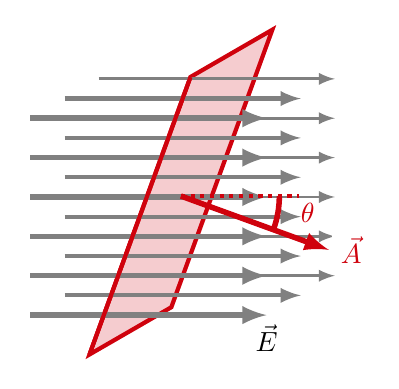
\begin{tikzpicture}
\tikzmath{
\thp=30;%perspective angle
\th=70;%tilt angle
\L=3;
}
\scalebox{1}{

%flux surface
\coordinate (P1) at ($(0.25*\L,-0.5)$);
\coordinate (P2) at ($(P1)+(\th:1.25*\L)$);
\coordinate (P3) at ($(P2)+(\thp:0.4*\L)$);
\coordinate (P4) at ($(P1)+(\thp:0.4*\L)$);
\coordinate (PC) at ($(P1)+(\th:1.25*\L/2)+(\thp:0.4*\L/2)$);
\draw [color=myred,line width=1.5] (P1) -- (P2) -- (P3) -- (P4) --cycle;
\fill[color=myred,opacity=0.2,draw =myred, line width=1.5] (P1) -- (P2) -- (P3) -- (P4) --cycle;
%field lines
\foreach \h in {0,0.5,...,2.5}{
 \draw[-latex, line width =2,color=black!50] (0,\h) -- +(\L,0);
 \draw[-latex, line width =1.5,color=black!50] ($(0,\h)+(\thp:0.5)$) -- +(\L,0);
 \draw[-latex, line width =1,color=black!50] ($(0,\h)+(\thp:1)$) -- +(\L,0);
}
%surface front line
\draw [color=myred,line width=1.5] (P1) -- (P2);
\draw[-latex, line width=2,color=myred] ($(PC)+(0,-0.05)$) -- +(\th-90:2) node[right,fill=white]{$\vec A$};
\draw[dotted,line width=1.5,color=myred]  ($(PC)+(0,-0.05)$) -- +(1.5,0);
\draw[line width=2,color=myred] ($(PC)+(1.25,-0.05)$) arc (0:\th-90:1.25) node[midway,right=4pt]{$\theta$};

\node[below] at (\L,0) {$\vec E$};
}

\end{tikzpicture}
\captionof*{figure}{\textit{Flux through an open surface.}}
\end{center}

}

%%%%%%%%%%%%%%%%%%%%%%%%%%%%%%

%%%%%%%%%%%%%%%%%%%%%%%%%%%%%%
\begin{frame}{Flux through a surface}
\vspace{-0.75cm}
\begin{align*}
\Phi_E=\vec E \cdot \vec A=EA\cos\theta
\end{align*}
\vspace{-0.5cm}
\begin{itemize}
 \item This definition of flux meets the requirements for the analogy with pellets or field lines:
 \begin{itemize}
 \item If the surface is perpendicular to the field, the most field lines cross the surface.
 \item If the surface is parallel to the field, no field lines cross the surface.
 \item If the electric field is stronger, more field lines cross the surface.
 \end{itemize}
 \item \textbf{For a closed surface, we define the direction of $\vec A$  to be outwards}.
 \end{itemize}
\vspace{-1.5cm} 
\begin{center}
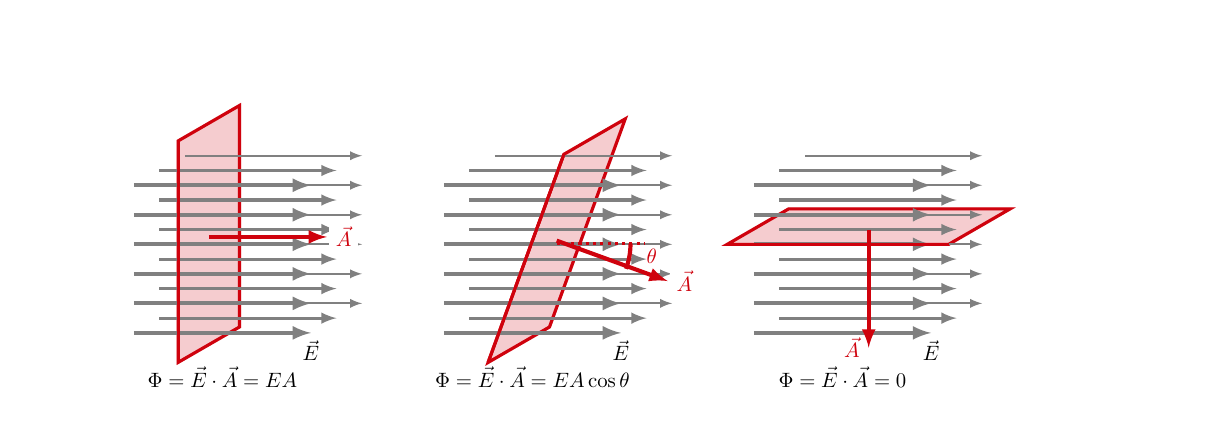
\begin{tikzpicture}[scale=1]
\tikzmath{
\thp=30;%perspective angle
\th=70;%tilt angle
\L=3;
}
\scalebox{0.75}{

%flux surface
\coordinate (P1) at ($(0.25*\L,-0.5)$);
\coordinate (P2) at ($(P1)+(\th:1.25*\L)$);
\coordinate (P3) at ($(P2)+(\thp:0.4*\L)$);
\coordinate (P4) at ($(P1)+(\thp:0.4*\L)$);
\coordinate (PC) at ($(P1)+(\th:1.25*\L/2)+(\thp:0.4*\L/2)$);
\draw [color=myred,line width=1.5] (P1) -- (P2) -- (P3) -- (P4) --cycle;
\fill[color=myred,opacity=0.2,draw =myred, line width=1.5] (P1) -- (P2) -- (P3) -- (P4) --cycle;
%field lines
\foreach \h in {0,0.5,...,2.5}{
 \draw[-latex, line width =2,color=black!50] (0,\h) -- +(\L,0);
 \draw[-latex, line width =1.5,color=black!50] ($(0,\h)+(\thp:0.5)$) -- +(\L,0);
 \draw[-latex, line width =1,color=black!50] ($(0,\h)+(\thp:1)$) -- +(\L,0);
}
%surface front line
\draw [color=myred,line width=1.5] (P1) -- (P2);
\draw[-latex, line width=2,color=myred] (PC) -- +(\th-90:2) node[right,fill=white]{$\vec A$};
\draw[dotted,line width=1.5,color=myred]  ($(PC)+(0,-0.05)$) -- +(1.5,0);
\draw[line width=2,color=myred] ($(PC)+(1.25,-0.05)$) arc (0:\th-90:1.25) node[midway,right=4pt]{$\theta$};

\node[below] at (\L,0) {$\vec E$};
\node at (0.5*\L,-0.75){$\Phi=\vec E\cdot \vec A=EA\cos\theta$};

\begin{scope}[shift={(-1.75*\L,0)}]
\tikzmath{\th=90;}
%flux surface
\coordinate (P1) at ($(0.25*\L,-0.5)$);
\coordinate (P2) at ($(P1)+(\th:1.25*\L)$);
\coordinate (P3) at ($(P2)+(\thp:0.4*\L)$);
\coordinate (P4) at ($(P1)+(\thp:0.4*\L)$);
\coordinate (PC) at ($(P1)+(\th:1.25*\L/2)+(\thp:0.4*\L/2)$);
\draw [color=myred,line width=1.5] (P1) -- (P2) -- (P3) -- (P4) --cycle;
\fill[color=myred,opacity=0.2,draw =myred, line width=1.5] (P1) -- (P2) -- (P3) -- (P4) --cycle;
%field lines
\foreach \h in {0,0.5,...,2.5}{
 \draw[-latex, line width =2,color=black!50] (0,\h) -- +(\L,0);
 \draw[-latex, line width =1.5,color=black!50] ($(0,\h)+(\thp:0.5)$) -- +(\L,0);
 \draw[-latex, line width =1,color=black!50] ($(0,\h)+(\thp:1)$) -- +(\L,0);
}
%surface front line
\draw [color=myred,line width=1.5] (P1) -- (P2);
\draw[-latex, line width=2,color=myred] ($(PC)+(0,-0.05)$) -- +(\th-90:2) node[right,fill=white]{$\vec A$};
%\draw[dotted,line width=1.5,color=myred]  ($(PC)+(0,-0.05)$) -- +(1.5,0);
%\draw[line width=2,color=myred] ($(PC)+(1.25,-0.05)$) arc (0:\th-90:1.25) node[midway,right=4pt]{$\theta$};
\node[below] at (\L,0) {$\vec E$};
\node at (0.5*\L,-0.75){$\Phi=\vec E\cdot \vec A=EA$};

\end{scope}

\begin{scope}[shift={(1.75*\L,0)}]
\tikzmath{\th=0;}
%flux surface
\coordinate (P1) at ($(0.25*\L,-0.5)+(-0.4*\L,2)$);
\coordinate (P2) at ($(P1)+(\th:1.25*\L)$);
\coordinate (P3) at ($(P2)+(\thp:0.4*\L)$);
\coordinate (P4) at ($(P1)+(\thp:0.4*\L)$);
\coordinate (PC) at ($(P1)+(\th:1.25*\L/2)+(\thp:0.4*\L/2)$);
\draw [color=myred,line width=1.5] (P1) -- (P2) -- (P3) -- (P4) --cycle;
\fill[color=myred,opacity=0.2,draw =myred, line width=1.5] (P1) -- (P2) -- (P3) -- (P4) --cycle;
%field lines
\foreach \h in {0,0.5,...,2.5}{
 \draw[-latex, line width =2,color=black!50] (0,\h) -- +(\L,0);
 \draw[-latex, line width =1.5,color=black!50] ($(0,\h)+(\thp:0.5)$) -- +(\L,0);
 \draw[-latex, line width =1,color=black!50] ($(0,\h)+(\thp:1)$) -- +(\L,0);
}
%surface front line
\draw [color=myred,line width=1.5] (P1) -- (P2);
\draw[-latex, line width=2,color=myred] ($(PC)+(0,-0.05)$) -- +(\th-90:2) node[left]{$\vec A$};
%\draw[dotted,line width=1.5,color=myred]  ($(PC)+(0,-0.05)$) -- +(1.5,0);
%\draw[line width=2,color=myred] ($(PC)+(1.25,-0.05)$) arc (0:\th-90:1.25) node[midway,right=4pt]{$\theta$};
\node[below] at (\L,0) {$\vec E$};
\node at (0.5*\L,-0.75){$\Phi=\vec E\cdot \vec A=0$};
\end{scope}
}

\end{tikzpicture}
\vspace{-0.75cm}
\captionof*{figure}{\textit{Flux through an open surface.}}
\end{center}

\end{frame}

%%%%%%%%%%%%%%%%%%%%%%%%%%%%%%
\twocolframe{Flux through a surface and scalar product}
{
\begin{align*}
\Phi_E=\vec E \cdot \vec A=EA\cos\theta
\end{align*}
\begin{itemize}
\item The scalar product ``selects'' the part of the surface vector that is parallel to the field: $A_\perp=A\cos\theta$.
\item The scalar product ``selects'' the part of the field that is parallel to the surface vector: $E_\perp=E\cos\theta$.
\end{itemize}
}
{
\begin{center}
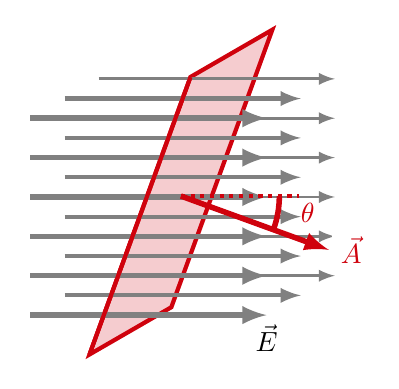
\begin{tikzpicture}
\tikzmath{
\thp=30;%perspective angle
\th=70;%tilt angle
\L=3;
}
\scalebox{1}{

%flux surface
\coordinate (P1) at ($(0.25*\L,-0.5)$);
\coordinate (P2) at ($(P1)+(\th:1.25*\L)$);
\coordinate (P3) at ($(P2)+(\thp:0.4*\L)$);
\coordinate (P4) at ($(P1)+(\thp:0.4*\L)$);
\coordinate (PC) at ($(P1)+(\th:1.25*\L/2)+(\thp:0.4*\L/2)$);
\draw [color=myred,line width=1.5] (P1) -- (P2) -- (P3) -- (P4) --cycle;
\fill[color=myred,opacity=0.2,draw =myred, line width=1.5] (P1) -- (P2) -- (P3) -- (P4) --cycle;
%field lines
\foreach \h in {0,0.5,...,2.5}{
 \draw[-latex, line width =2,color=black!50] (0,\h) -- +(\L,0);
 \draw[-latex, line width =1.5,color=black!50] ($(0,\h)+(\thp:0.5)$) -- +(\L,0);
 \draw[-latex, line width =1,color=black!50] ($(0,\h)+(\thp:1)$) -- +(\L,0);
}
%surface front line
\draw [color=myred,line width=1.5] (P1) -- (P2);
\draw[-latex, line width=2,color=myred] ($(PC)+(0,-0.05)$) -- +(\th-90:2) node[right,fill=white]{$\vec A$};
\draw[dotted,line width=1.5,color=myred]  ($(PC)+(0,-0.05)$) -- +(1.5,0);
\draw[line width=2,color=myred] ($(PC)+(1.25,-0.05)$) arc (0:\th-90:1.25) node[midway,right=4pt]{$\theta$};

\node[below] at (\L,0) {$\vec E$};
}

\end{tikzpicture}
\captionof*{figure}{\textit{Flux through an open surface. $A\cos\theta$ is the part of $\vec A$ that is parallel to $\vec E$.}}
\end{center}
}


%%%%%%%%%%%%%%%%%%%%%%%%%%%%%%
\subsection{Calculating changes in flux across a surface}
\label{subsec:calculatingchangesinfluxacrossasurface}
\twocolframesf{What if the field changes across the surface?}
{
\begin{itemize}
\item If the field is different across each point on the surface, need to break the surface up into smaller surface elements, where the field is constant:
\begin{itemize}
\item The direction of $\vec E$ can change with respect to the surface normal.
\item The magnitude of $\vec E$ can change.
\end{itemize}
\item \textbf{The flux through the total surface is the sum of the fluxes through each surface element}:
\begin{align*}
\Phi=\Phi_1+\Phi_2+\Phi_3
\end{align*}
\end{itemize}
}
{

\begin{center}
\begin{tikzpicture}
\tikzmath{
\thp=30;%perspective angle
\L=3;
}
\scalebox{1}{

%flux surface
\coordinate (P1) at ($(0,0)$);
\coordinate (P2) at ($(P1)+(\thp:0.75*\L)$);
\coordinate (P3) at ($(P2)+(\L,0)$);
\coordinate (P4) at ($(P1)+(\L,0)$);
\draw [color=myred,line width=1.5] (P1) -- (P2) -- (P3) -- (P4) --cycle;
\fill[color=myred,opacity=0.2,draw =myred, line width=1.5] (P1) -- (P2) -- (P3) -- (P4) --cycle;


%elements
\coordinate (P5) at ($(P1)+(\thp:0.25*\L)+(\L/3,0)$);
\coordinate (P6) at ($(P5)+(\thp:0.25*\L)+(\L/3,0)$);
\fill [color=myred, opacity=0.5, line width=1.5, draw=myred!50!black] (P1) -- ($(P1)+(\thp:0.25*\L)$) -- (P5) -- ($(P1)+(\L/3,0)$) ;
\fill [color=myred, opacity=0.5, line width=1.5, draw=myred!50!black] (P5) -- ($(P5)+(\thp:0.25*\L)$) -- (P6) -- ($(P5)+(\L/3,0)$) -- cycle;
\fill [color=myred, opacity=0.5, line width=1.5, draw=myred!50!black] (P6) -- ($(P6)+(\thp:0.25*\L)$) -- (P3) -- ($(P6)+(\L/3,0)$) -- cycle;

%centres
\coordinate (Pc1) at ($(P1)+0.5*(\thp:0.25*\L)+0.5*(\L/3,0)$);
\coordinate (Pc2) at ($(P5)+0.5*(\thp:0.25*\L)+0.5*(\L/3,0)$);
\coordinate (Pc3) at ($(P3)-0.5*(\thp:0.25*\L)-0.5*(\L/3,0)$);

%field lines
\only<1>{
\draw[-latex, line width=1.5, color=black!50] ($(Pc1)+(0:0.2)$) -- +(0,0.75*\L);
\draw[-latex, line width=1.5, color=black!50] ($(Pc1)+(0:-0.2)$) -- +(0,0.75*\L) node[above]{$3E$};
\draw[-latex, line width=1.5, color=black!50] ($(Pc1)+(240:0.2)$) -- +(0,0.75*\L);

\draw[-latex, line width=1.5, color=black!50] ($(Pc2)+(0:0.2)$) -- +(0,0.75*\L);
\draw[-latex, line width=1.5, color=black!50] ($(Pc2)+(0:-0.2)$) -- +(0,0.75*\L) node[above]{$2E$};

\draw[-latex, line width=1.5, color=black!50] ($(Pc3)+(0:0.2)$) -- +(0,0.75*\L) node[above]{$E$};

\draw[-latex, color=myred, line width=2] (Pc1) -- +(0,1) node[above, fill=white, fill opacity=0.6]{$d\vec A$};
\draw[-latex, color=myred, line width=2] (Pc2) -- +(0,1) node[above, fill=white, fill opacity=0.6]{$d\vec A$};
\draw[-latex, color=myred, line width=2] (Pc3) -- +(0,1) node[above, fill=white, fill opacity=0.6]{$d\vec A$};
}

\only<2>{

  \foreach \th in {30,45,..., 150}{
    \draw[-latex, line width=1.5, color=black!50]  ($(Pc2)-(0,1)$) -- +(\th:3); 
  }
  \draw[-latex, color=myred, line width=2] (Pc1) -- +(0,1) node[above, fill=white, fill opacity=0.6]{$d\vec A$};
  \draw[-latex, color=myred, line width=2] (Pc2) -- +(0,1) node[above, fill=white, fill opacity=0.6]{$d\vec A$};
  \draw[-latex, color=myred, line width=2] (Pc3) -- +(0,1) node[above, fill=white, fill opacity=0.6]{$d\vec A$};
  \node[above right, color=black!50] at  ($(Pc2)+(0,2)$) {$\vec E$}; 
  }
}

\end{tikzpicture}
\captionof*{figure}{\textit{Dividing a surface into smaller elements when the $\vec E \cdot \vec A$ changes across the surface.}}
\end{center}
}

%%%%%%%%%%%%%%%%%%%%%%%%%%%%%%
\begin{bulletframe}{More general definition of flux}
\item In general, if the field varies continuously over the surface S, we need to \textbf{take infinitessimally small area elements, $ d\vec A$,} and sum (integrate) the infinitely many fluxes from each area element.
\item The flux becomes (a 2D ``surface integral''):
\begin{align*}
\Phi_E=\int_S \vec E \cdot d\vec A
\end{align*}
\item \textbf{Think of adding together a bunch of little fluxes}, $d\Phi$:
\begin{align*}
d\Phi = \vec E \cdot d\vec A
\end{align*}
\item The subscript S indicates that we are integrating over the 2D surface, S. In general, this is a “double integral” and rather painful to solve, \textit{so we want to avoid having to actually do the integral!}
\begin{align*}
\int_S \vec E \cdot d\vec A = \int\int E(x,y)\cos\theta(x,y)dxdy
\end{align*}
\end{bulletframe}



%%%%%%%%%%%%%%%%%%%%%%%%%%%%%%
\twocolframesf{Strategy for the flux integral}
{
\begin{itemize}
\item Remember, the integral is a sum, so we can break the integral over the whole surface into integrals over more convenient surfaces:
\begin{align*}
\Phi_E=\int_S \vec E \cdot d\vec A=\int_{S_1} \vec E \cdot d\vec A+\int_{S_2} \vec E \cdot d\vec A
\end{align*}
\item \textbf{We want to avoid doing an actual integral!}
\item We always try to break the surface up into sub surfaces over which the electric field is constant.
\item When we use Gauss’ Law, we can choose the surface, so we choose one where the integrals are easy!
\end{itemize}
}
{

\begin{center}
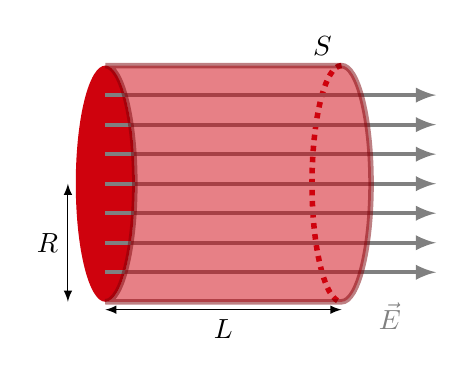
\begin{tikzpicture}
\tikzmath{
\R=1.5;
\L=3;
}
\scalebox{1}{

\fill[color=myred] (0,0) circle({\R/4} and \R);
\draw[dotted, color=myred, line width=2] (\L,\R) arc(90:270:{\R/4} and \R);

\foreach \i in {-0.75,-0.5,...,0.75}{
  \draw[-latex, line width=1.5, color=black!50] (0,\i*\R) -- +(1.4*\L,0);
}
%body
\fill[color=myred,opacity=0.5, draw =myred!60!black, line width=2] (0,\R) -- (\L,\R) arc(90:-90:{\R/4} and \R) -- (0,-\R) arc (-90:90:{\R/4} and \R);

\node[above left] at (\L,\R) {$S$};

\node[below=5pt, right=10pt,color=black!50] at (\L,-\R) {$\vec E$};
\draw[latex-latex] (0,-\R-0.1) -- +(\L,0) node[midway,below]{$L$};
\draw[latex-latex] (-\R/4-0.1,-\R) -- +(0,\R) node[midway,left]{$R$};
}

\end{tikzpicture}
\captionof*{figure}{\textit{Flux through a closed cylinder.}}
\end{center}

}

%%%%%%%%%%%%%%%%%%%%%%%%%%%%%%





\section{Application of Gauss's Law}
\label{sec:applicationofgaussslaw}
\title{Application of Gauss's Law}


%%%%%%%%%%%%%%%%%%%%%%%%%
\begin{frame}
\titlepage
\thispagestyle{empty}
\end{frame}

%





%%%%%%%%%%%%%%%%%%%%%%%%%%%%%%
\subsection{Using Gauss's Law}
\label{subsec:usinggaussslaw}
\begin{bulletframe}{Using Gauss' Law}
\item Only practical to use when we can actually calculate the flux (do the integral):
\begin{align*}
\Phi_E=\oint_S \vec E \cdot d\vec A=\oint_{S}E\cos\theta dA 
\end{align*}
\item This means \textbf{choosing a clever surface}:
\begin{itemize}
\item One that goes through a point where we want to know the electric field (kinda the point).
\item One where $\vec E$ is constant, ideally, or, 
\item One where $\vec E$ is constant in magnitude.
\item One where we can calculate its area easily:
\begin{align*}
\Phi_E=E\cos\theta \oint_S dA =E\cos\theta A
\end{align*}
\end{itemize}
\item The integral is only ever easy if the problem has a high degree of symmetry.
\end{bulletframe}


%%%%%%%%%%%%%%%%%%%%%%%%%%%%%%%%
\subsection{Field outside a charged sphere}
\label{subsec:fieldoutsideachargedsphere}
\twocolframesf{Field outside of sphere of radius, $R$, carrying charge $Q$}
{
Want the field, $\vec E(\vec r)$, at some distance $r$ from the centre:
\only<1>{
Need to \textbf{choose a Gaussian surface} that has:
 \begin{itemize}
  \item $\vec E$ always parallel or perpendicular to it.
  \item $\vec E$ constant in magnitude.
 \end{itemize}
 }
\begin{itemize}
\item[1]<2-> Choose a spherical surface ($S$) of radius $r$.
\only<3,4>{
\item[2] Evaluate the flux integral (use symmetry arguments):
\begin{align*}
\oint \vec E(\vec r) \cdot d\vec A=\oint E(r) dA=E(r) \oint dA
\end{align*}

\item[$\rightarrow$]<4> Adding together all of the $dA$:
\begin{align*}
\oint dA&=4\pi r^2\\
\therefore \oint \vec E(\vec r) \cdot d\vec A&=4\pi r^2 E(r)
\end{align*}
}
\only<5>{
\item[2] Evaluate the flux integral: $4\pi r^2 E(r)$\\
\item[3] Determine the charge enclosed. In this case, all of $Q$ is enclosed:
\begin{align*}
Q^{enc}=Q
\end{align*}
}
\only<6>{
\item[2] Evaluate the flux integral: $-4\pi r^2 E(r)$
\item[3] Determine the charge enclosed: $Q^{enc}=Q$
\item[4] Put it all together:
\begin{align*}
\oint \vec E(\vec r) \cdot d\vec A&=\frac{ Q^{enc}}{\epsilon_0}\\
4\pi r^2 E(r) &= \frac{ Q}{\epsilon_0} \\
\therefore\;\;\Aboxed{ E(r)&= \frac{1}{4\pi\epsilon_0}\frac{Q}{r^2} }
\end{align*}
}
\end{itemize}

}
{
\begin{center}
\begin{tikzpicture}
\tikzmath{
\Rm=0.3;
\Rs=1.5;
}
\scalebox{1}{

\shade[ball color=myblue!60] (0,0,0) circle (\Rm);
\only<1>{\node at (-45:2.5*\Rm) {\scriptsize $Q,R$};}
\fill (-\Rs,0) circle(2pt);
\draw[dashed,line width=1] (0,0) -- (-\Rs,0) node[midway,above]{$r$};

\only<2->{
\draw[-latex, line width=1] ($(45:0.775*\Rs)+(-0.05,0.05) $) -- +(45:0.75) node[left=5pt]{$\vec E$};
\shade[ball color=myred, opacity=0.25] (0,0,0) circle (\Rs);
\draw[line width=1.5, color=myred, opacity=0.5] (\Rs,0) arc(0:-180:{\Rs} and {\Rs/4});
\node[color=myred] at (135:1.5*\Rs){$S$};

\fill[color=myred,opacity=0.5, draw=black] (35:0.7*\Rs) -- (37.5:0.85*\Rs) -- (52.5:0.85*\Rs) -- (55:0.7*\Rs) --cycle;
\draw[-latex,color=myred, line width=1] (45:0.775*\Rs) -- +(45:0.75) node[right]{$d\vec A$};
}
}
\end{tikzpicture}
\captionof*{figure}{\textit{Gauss' Law to find field outside of a spherical charge of radius, $R$, and charge, $Q$.}}
\end{center}
}








%%%%%%%%%%%%%%%%%%%%%%%%%%%%
\subsection{Steps to using Gauss's law}
\label{subsec:stepstousinggaussslaw}
\begin{frame}{Steps to Using Gauss' Law}
\begin{align*}
\Phi_E =\frac{Q^{enc}}{\epsilon_0}
\end{align*}
Three steps:
\begin{enumerate}
\item Calcuate the flux.
\item Calculate the charge enclosed.
\item Put it all together.
\end{enumerate}
\end{frame}


%%%%%%%%%%%%%%%%%%%%%%%%%%%%%%%%
\begin{bulletframe}{Using Gauss' Law}
\item Only practical to use when we can actually calculate the flux (do the integral):
\begin{align*}
\Phi_E=\oint_S \vec E \cdot d\vec A=\oint_{S}E\cos\theta dA 
\end{align*}
\item This means \textbf{choosing a clever surface}:
\begin{itemize}
\item One that goes through a point where we want to know the electric field (kinda the point).
\item One where $\vec E$ is constant, ideally  or 
\item One where $\vec E$ is constant in magnitude.
\item One where we can calculate its area easily:
\begin{align*}
\Phi_E=E\cos\theta \oint_S dA =E\cos\theta A
\end{align*}
\end{itemize}
\item The integral is only ever easy if the problem has a high degree of symmetry.
\end{bulletframe}


%%%%%%%%%%%%%%%%%%%%%%%%%%%%%%%%
\twocolframesf{Recall: Field outside of sphere of radius, $R$, carrying charge $Q$}
{
Want the field, $\vec E(\vec r)$, at some distance $r$ from the centre:
\begin{itemize}
\item[1] Choose a spherical surface ($S$) of radius $r$.
\item[2] Evaluate the flux integral: $4\pi r^2 E(r)$
\item[3] Determine the charge enclosed: $Q^{enc}=Q$
\item[4] Put it all together:
\begin{align*}
\oint \vec E(\vec r) \cdot d\vec A&=\frac{ Q^{enc}}{\epsilon_0}\\
4\pi r^2 E(r) &= \frac{ Q}{\epsilon_0} \\
\therefore\;\;\Aboxed{ E(r)&= \frac{1}{4\pi\epsilon_0}\frac{Q}{r^2} }
\end{align*}

\end{itemize}

}
{
\begin{center}
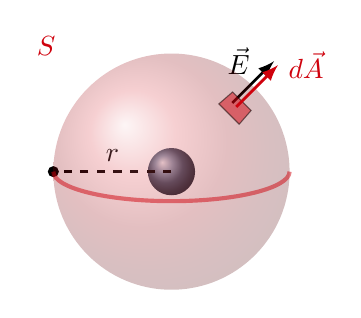
\begin{tikzpicture}
\tikzmath{
\Rm=0.3;
\Rs=1.5;
}
\scalebox{1}{

\shade[ball color=myblue!60] (0,0,0) circle (\Rm);
\fill (-\Rs,0) circle(2pt);
\draw[dashed,line width=1] (0,0) -- (-\Rs,0) node[midway,above]{$r$};

\draw[-latex, line width=1] ($(45:0.775*\Rs)+(-0.05,0.05) $) -- +(45:0.75) node[left=5pt]{$\vec E$};
\shade[ball color=myred, opacity=0.25] (0,0,0) circle (\Rs);
\draw[line width=1.5, color=myred, opacity=0.5] (\Rs,0) arc(0:-180:{\Rs} and {\Rs/4});
\node[color=myred] at (135:1.5*\Rs){$S$};

\fill[color=myred,opacity=0.5, draw=black] (35:0.7*\Rs) -- (37.5:0.85*\Rs) -- (52.5:0.85*\Rs) -- (55:0.7*\Rs) --cycle;
\draw[-latex,color=myred, line width=1] (45:0.775*\Rs) -- +(45:0.75) node[right]{$d\vec A$};

}
\end{tikzpicture}
\captionof*{figure}{\textit{Gauss' Law to find field outside of a spherical charge of radius, $R$, and charge, $Q$.}}
\end{center}
}


%%%%%%%%%%%%%%%%%%%%%%%%%%%%%%%%
\subsection{Field inside a charged sphere}
\label{subsec:fieldinsideachargedsphere}
\twocolframesf{Field \textit{inside} of a uniform sphere of radius, $R$, and charge, $Q$}
{
Want the field, $\vec E(\vec r)$, at some distance $r$ from the centre:
\only<1>{
\newline
}
\begin{itemize}
\item[1]<2-> Choose a spherical surface ($S$) of radius $r<R$.
\only<3>{
\item[2] Evaluate the flux integral (same as before):
\begin{align*}
\oint \vec E(\vec r) \cdot d\vec A&=\oint E(r) dA=E(r) \oint dA\\
&=4\pi r^2 E(r)
\end{align*}
}
\only<4>{
\item[2] Evaluate the flux integral: $4\pi r^2 E(r)$
\item[3] Determine the charge enclosed. Use the charge density, $\rho=\frac{Q}{V}$:
\begin{align*}
\rho&=\frac{Q}{\frac{4}{3}\pi R^3}\\
Q^{enc}&=\rho \frac{4}{3}\pi r^3=\frac{Q}{\frac{4}{3}\pi R^3}\frac{4}{3}\pi r^3\\
&=Q\frac{r^3}{R^3}
\end{align*}
}
\only<5>{
\item[2] Evaluate the flux integral: $-4\pi r^2 g(r)$
\item[3] Determine the mass enclosed: $Q^{enc}=Q\frac{r^3}{R^3}$
\item[4] Put it all together:
\begin{align*}
\oint \vec E(\vec r) \cdot d\vec A&=\frac{Q^{enc}}{\epsilon_0}\\
4\pi r^2 E(r) &= \frac{Q}{\epsilon_0}\frac{r^3}{R^3} \\
\therefore E(r)&=\frac{Q}{4\pi\epsilon_0R^3}r
\end{align*}
}
\end{itemize}

}
{
\begin{center}
\begin{tikzpicture}
\tikzmath{
\Rm=2;
\Rs=1.25;
}
\scalebox{1}{
\draw[dashed,line width=1] (0,0) -- (-\Rs,0) node[midway,above]{$r$};
\fill (-\Rs,0) circle(2pt);
\only<1>{
\shade[ball color=myblue!60,opacity=0.5] (0,0,0) circle (\Rm);
}
\node at (-45:1.15*\Rm) {\scriptsize $Q,R$};


\only<2->{
\draw[-latex, line width=1] ($(45:0.775*\Rs)+(-0.05,0.05) $) -- +(45:0.75) node[left=5pt]{$\vec E$};
%\draw[-latex, line width=1] (45:0.775*\Rs) -- +(45:-0.75) node[right=5pt]{$\vec g$};
\shade[ball color=myred, opacity=0.25] (0,0,0) circle (\Rs);
\draw[line width=1.5, color=myred, opacity=0.5] (\Rs,0) arc(0:-180:{\Rs} and {\Rs/4});
\node[color=myred] at (135:1.25*\Rs){$S$};

\fill[color=myred,opacity=0.6, draw=black] (35:0.7*\Rs) -- (37.5:0.85*\Rs) -- (52.5:0.85*\Rs) -- (55:0.7*\Rs) --cycle;

\draw[-latex,color=myred, line width=1] (45:0.775*\Rs) -- +(45:0.75) node[right]{$d\vec A$};
\shade[ball color=myblue!60,opacity=0.5] (0,0,0) circle (\Rm);
}

}

\end{tikzpicture}
\captionof*{figure}{\textit{Gauss' Law to find field inside of a spherical charge, $Q$, of radius.}}
\end{center}
\only<5>{
Inside the sphere, the field increases linearly with radius. Outside it decreases with $r^2$.
}
}

%%%%%%%%%%%%%%%%%%%%%%%%%%%%%%%%


%%%%%%%%%%%%%%%%%%%%%%%%%%%%%%%%
\subsection{Field near an infinitely long charged wire}
\label{subsec:fieldnearaninfinitelylongchargedwire}
\twocolframesf{Field near an infinitely long charged wire}
{
We want to know the electric field at a distance, $r$, from an infinitely long wire carrying charge per unit length, $\lambda$. We know how to do this with an integral (lecture 45):
\begin{align*}
E(r) = \frac{\lambda r}{4\pi\epsilon_0} \int_{-\infty}^{+\infty}\frac{dy}{\left(y^2+r^2\right)^{\frac{3}{2}}}
\end{align*}
... actually not too bad if you use $\theta$ instead of $y$ (trig substitution)!
}
{
\begin{center}
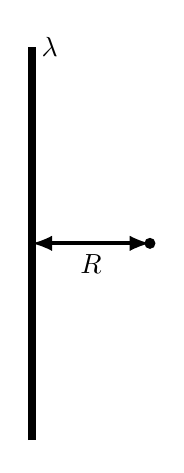
\begin{tikzpicture}
\tikzmath{
\L=5;
\R=1.5;
}
\scalebox{1}{
\draw[line width=3] (0,-\L/2) -- (0,\L/2);
\fill (\R,0) circle (2pt);
\draw[latex-latex, line width=1.5] (0,0) -- (\R, 0) node[midway,below]{$R$};
\node[right] at (0,\L/2) {$\lambda$};
}


\end{tikzpicture}
\captionof*{figure}{\textit{An infinite wire carrying uniform charge per unit length, $\lambda$.}}
\end{center}
}

%%%%%%%%%%%%%%%%%%%%%%%%%%%%%%%%




%%%%%%%%%%%%%%%%%%%%%%%%%%%%%%%%
\twocolframesf{Field near an infinitely long charged wire}
{
\only<1>{
We choose a cylindrical gaussian surface of length, $L$, and radius, $r$, such that it passes through the point where we want to know the electric field.
\newline
}
\only<2>{
\begin{itemize}
\item[1] Choose a cylindrical gaussian surface.
\item[2] Calculate flux through the surface:
\begin{itemize}
  \item Break the surface into:
  \begin{enumerate}
    \item Endcaps:
    \begin{align*}
    \Phi_{endcaps} = 0
    \end{align*}
    There are no field lines crossing the endcap.
    \item Wrap-around:
    \begin{align*}
    \Phi_{wraparound} = \oint_S \vec E \cdot d\vec A = E \oint_S dA =E(2\pi rL)
    \end{align*}
    You can ``unwrap'' into a rectangle of height $L$ and length $2\pi R$.
  \end{enumerate}
\end{itemize} 
\end{itemize}
}
\only<3->{
\begin{itemize}
\item[1] Choose a cylindrical gaussian surface.
\item[2] Calculate flux through the surface: $\Phi=E(2\pi rL)$
\item[3] Calculate the charge enclosed: $Q^{enc}=\lambda L$
\item<4>[4] Putting it all together:
\begin{align*}
\oint \vec E(\vec r) \cdot d\vec A&=\frac{Q^{enc}}{\epsilon_0}\\
E(2\pi rL) &= \frac{\lambda L}{\epsilon_0}\quad\text{The $L$ cancels!}\\
\therefore E(r)&=\frac{\lambda}{2\pi\epsilon_0R}
\end{align*}
\end{itemize}

}

}
{
\begin{center}
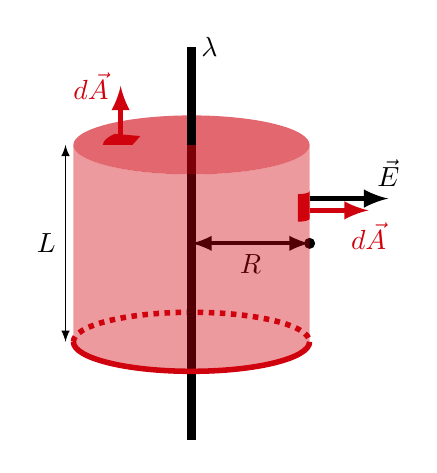
\begin{tikzpicture}
\tikzmath{
\L=5;
\R=1.5;
\r=0.5*\R;
\dr=0.25*\R;
\rpdr=\r+\dr;
}
\scalebox{1}{
\fill (\R,0) circle (2pt);
\draw[latex-latex, line width=1.5] (0,0) -- (\R, 0) node[midway,below]{$R$};
\node[right] at (0,\L/2) {$\lambda$};

\draw[line width=2, dotted, color=myred] (-\R,-\L/4) arc (180:0:{\R} and {\R/4});
\draw[line width=3] (0,-\L/2) -- (0,\L/4);
\fill[color=myred, opacity=0.6] (0,\L/4) circle({\R} and {\R/4});
\draw[line width=3] (0,\L/4) -- (0,\L/2);
\fill[color=myred, opacity=0.4] (\R,\L/4) -- (\R,-\L/4) arc (0:-180:{\R} and {\R/4}) -- (-\R,\L/4) arc (-180:0:{\R} and {\R/4});
\draw[line width=2, color=myred] (-\R,-\L/4) arc (-180:0:{\R} and {\R/4});
\draw[latex-latex] (-\R-0.1,-\L/4) -- +(0,\L/2) node[midway,left]{$L$};

\only<2->{
  \fill[color=myred] (\R,\L/8) -- (\R,0.5*\L/8) arc (0:-90:{0.1*\R} and {0.1*\R/4}) -- (0.9*\R,\L/8) arc(-90:0:{0.1*\R} and {0.1*\R/4});
  \draw[-latex, color=myred,line width=2] (\R,0.75*\L/8-0.05) -- +(0.75,0)node[below]{$d\vec A$};
  \draw[-latex, line width=2] (\R,0.75*\L/8+0.1) -- +(1,0)node[above]{$\vec E$};
  
  \coordinate (P1) at ($(0,\L/4)+(180:\r)$);
  \coordinate (P2) at ($(0,\L/4)+(180:\rpdr)$);
  \coordinate (P4) at ($(0,\L/4)+(150:\r)-(0,0.35*\r)$);
  \fill[color=myred] (P1) -- (P2) arc(180:150:{\rpdr} and {\rpdr/4} ) -- (P4) -- (P1);
  \draw[-latex, color=myred,line width=2] ($(0,\L/4)+(-0.6*\R,0)$) -- +(0,0.75)node[left]{$d\vec A$};  
}

}
\end{tikzpicture}
\captionof*{figure}{\textit{An infinite wire carrying uniform charge per unit length, $\lambda$.}}
\end{center}
}

%%%%%%%%%%%%%%%%%%%%%%%%%%%%%%%
\subsection{Field from infinite plane of charge}
\label{subsec:fieldfrominfiniteplaneofcharge}
\twocolframesf{Infinite plane of charge}
{
We want to know the electric field near an infinite plane carrying uniform charge per unit area, $\sigma$
}
{
\begin{center}
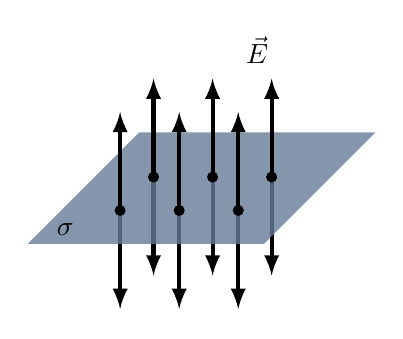
\begin{tikzpicture}
\tikzmath{
\L=3;
\Ly=2;
\thp=45;
}
\scalebox{1}{

\coordinate (P1) at (0,0);
\coordinate (P2) at ($(P1)+(\thp:\Ly)$);
\coordinate (P3) at ($(P2)+(0:\L)$);
\coordinate (P4) at ($(P1)+(0:\L)$);

\foreach \i in {0.3,0.6}{
\draw[-latex, line width=1.5,color=black] ($(P1)+(0.25*\L,0)+(\thp:\i*\Ly)$) -- +(0,-1.25) ;
\draw[-latex, line width=1.5,color=black] ($(P1)+(0.5*\L,0)+(\thp:\i*\Ly)$) -- +(0,-1.25) ;
\draw[-latex, line width=1.5,color=black] ($(P1)+(0.75*\L,0)+(\thp:\i*\Ly)$) -- +(0,-1.25) ;
}
\fill[color=myblue!60,opacity=0.8] (P1) -- (P2) -- (P3) -- (P4);
\foreach \i in {0.3,0.6}{
\draw[-latex, line width=1.5,color=black] ($(P1)+(0.25*\L,0)+(\thp:\i*\Ly)$) -- +(0,1.25) ;
\draw[-latex, line width=1.5,color=black] ($(P1)+(0.5*\L,0)+(\thp:\i*\Ly)$) -- +(0,1.25) ;
\draw[-latex, line width=1.5,color=black] ($(P1)+(0.75*\L,0)+(\thp:\i*\Ly)$) -- +(0,1.25) ;
\fill ($(P1)+(0.25*\L,0)+(\thp:\i*\Ly)$) circle (2pt);
\fill ($(P1)+(0.5*\L,0)+(\thp:\i*\Ly)$) circle (2pt);
\fill ($(P1)+(0.75*\L,0)+(\thp:\i*\Ly)$) circle (2pt);
}
\node[above=0.75cm] at ($(P2)!0.5!(P3)$){$\vec E$};

\node[above=5pt,right=7pt] at (P1) {$\sigma$};


}
\end{tikzpicture}
\captionof*{figure}{\textit{An infinite plane of charge, carrying charge per unit area, $\sigma$.}}
\end{center}
}


%%%%%%%%%%%%%%%%%%%%%%%%%%%%%%%%
\twocolframefs{Infinite plane of charge}
{
Two ``obvious'' choices of gaussian surface:
\begin{itemize}
\item Cylinder
\item Rectangular prism
\end{itemize}
}
{
\begin{center}
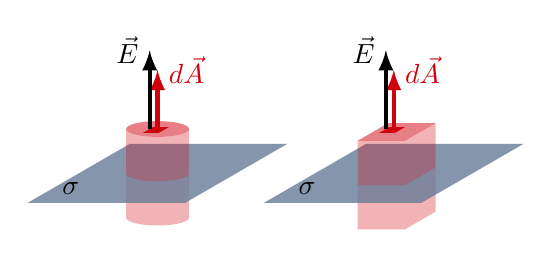
\begin{tikzpicture}
\tikzmath{
\L=2;
\fr=1.5/2;
\Ly=\L*\fr;
\thp=30;
\R=0.2*\L;
\h=0.75*\Ly;
\dax=0.5*\R;
\abox=1.5*\R;
}
\scalebox{1}{

\coordinate (P1) at ($(-\L/2,0) - (\thp:0.5*\Ly)$);
\coordinate (P2) at ($(P1)+(\thp:\Ly)$);
\coordinate (P3) at ($(P2)+(0:\L)$);
\coordinate (P4) at ($(P1)+(0:\L)$);

\fill[color=myred, opacity=0.3] (\R,0) -- (\R,-\h/2) arc (0:-180:{\R} and {\R/4}) -- (-\R,0) arc (-180:0:{\R} and {\R/4});
\fill[color=myblue!60,opacity=0.8] (P1) -- (P2) -- (P3) -- (P4);

\fill[color=myred, opacity=0.3] (\R,0) -- (\R,\h/2) arc (0:-180:{\R} and {\R/4}) -- (-\R,0) arc (-180:0:{\R} and {\R/4});
\fill[color=myred, opacity=0.5] (0,\h/2) circle({\R} and {\R/4});

\coordinate (P1a) at ($(-\dax/2,\h/2) - (\thp:0.5*\dax)$);
\coordinate (P2a) at ($(P1a)+(\thp:0.75*\dax)$);
\coordinate (P3a) at ($(P2a)+(0:\dax)$);
\coordinate (P4a) at ($(P1a)+(0:\dax)$);
\fill[color=myred] (P1a) -- (P2a) -- (P3a) -- (P4a);
\draw[-latex,color=myred,line width = 1.5] (0,\h/2) -- +(0,0.75) node[right]{$d\vec A$};
\draw[-latex,line width = 1.5] (-0.1,\h/2) -- +(0,1) node[left]{$\vec E$};
\node[above=5pt,right=9pt] at (P1) {$\sigma$};
\begin{scope}[shift={(1.5*\L,0)}]

%the plane:
\coordinate (P1) at ($(-\L/2,0) - (\thp:0.5*\Ly)$);
\coordinate (P2) at ($(P1)+(\thp:\Ly)$);
\coordinate (P3) at ($(P2)+(0:\L)$);
\coordinate (P4) at ($(P1)+(0:\L)$);

%the box
\coordinate (P1b) at ($(-\R/2,0) - (\thp:0.5*\abox)$);
\coordinate (P2b) at ($(P1b)+(\thp:0.75*\abox)$);
\coordinate (P3b) at ($(P2b)+(0:\abox)$);
\coordinate (P4b) at ($(P1b)+(0:\abox)$);


\fill[color=myred, opacity=0.3] (P1b) -- ($(P1b)-(0,\h/2)$) -- ($(P4b)-(0,\h/2)$) -- ($(P3b)-(0,\h/2)$) -- (P3b) -- (P4b) -- (P1b);
\fill[color=myblue!60,opacity=0.8] (P1) -- (P2) -- (P3) -- (P4);
\fill[color=myred, opacity=0.3] (P1b) -- ($(P1b)+(0,\h/2)$) -- ($(P4b)+(0,\h/2)$) -- ($(P3b)+(0,\h/2)$) -- (P3b) -- (P4b) -- (P1b);
\fill[color=myred, opacity=0.5] ($(P1b)+(0,\h/2)$) -- ($(P2b)+(0,\h/2)$) -- ($(P3b)+(0,\h/2)$) -- ($(P4b)+(0,\h/2)$) --cycle;

%dA and E:
\coordinate (P1a) at ($(-\dax/2,\h/2) - (\thp:0.5*\dax)$);
\coordinate (P2a) at ($(P1a)+(\thp:0.75*\dax)$);
\coordinate (P3a) at ($(P2a)+(0:\dax)$);
\coordinate (P4a) at ($(P1a)+(0:\dax)$);
\fill[color=myred] (P1a) -- (P2a) -- (P3a) -- (P4a);
\draw[-latex,color=myred,line width = 1.5] (0,\h/2) -- +(0,0.75) node[right]{$d\vec A$};
\draw[-latex,line width = 1.5] (-0.1,\h/2) -- +(0,1) node[left]{$\vec E$};
\node[above=5pt,right=9pt] at (P1) {$\sigma$};
\end{scope}
}
\end{tikzpicture}
\captionof*{figure}{\textit{Two options for gaussian surfaces to model the infinite plane.}}
\end{center}

}

%%%%%%%%%%%%%%%%%%%%%%%%%%%%%%%%
\twocolframesf{Infinite plane of charge}
{
Choosing the cylinder, we have:
\begin{itemize}
\item Flux is only through endcaps (there are two of them!):\\ $\Phi_E=\Phi_{endcaps}+\Phi_{wraparound}=\boldsymbol{2} E\pi r^2$
\item Charge enclosed by the surface:\\ $Q^{enc}=\sigma \pi r^2 $
\end{itemize}
All together:
\begin{align*}
\Phi_E =\frac{Q^{enc}}{\epsilon_0}\rightarrow \;\;\;
2E\pi r^2 &= \frac{\sigma \pi r^2}{\epsilon_0}\\
\therefore E&=\frac{\sigma}{2\epsilon_0}
\end{align*}
The electric field does not depend on distance from the plane, it's constant everywhere in space!
}
{
\begin{center}
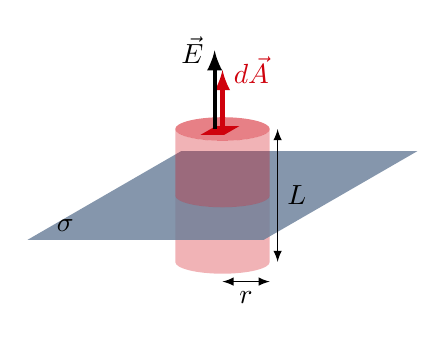
\begin{tikzpicture}
\tikzmath{
\L=3;
\fr=1.5/2;
\Ly=\L*\fr;
\thp=30;
\R=0.2*\L;
\h=0.75*\Ly;
\dax=0.5*\R;
}
\scalebox{1}{

\coordinate (P1) at ($(-\L/2,0) - (\thp:0.5*\Ly)$);
\coordinate (P2) at ($(P1)+(\thp:\Ly)$);
\coordinate (P3) at ($(P2)+(0:\L)$);
\coordinate (P4) at ($(P1)+(0:\L)$);

\fill[color=myred, opacity=0.3] (\R,0) -- (\R,-\h/2) arc (0:-180:{\R} and {\R/4}) -- (-\R,0) arc (-180:0:{\R} and {\R/4});
\fill[color=myblue!60,opacity=0.8] (P1) -- (P2) -- (P3) -- (P4);

\fill[color=myred, opacity=0.3] (\R,0) -- (\R,\h/2) arc (0:-180:{\R} and {\R/4}) -- (-\R,0) arc (-180:0:{\R} and {\R/4});
\fill[color=myred, opacity=0.5] (0,\h/2) circle({\R} and {\R/4});

\coordinate (P1a) at ($(-\dax/2,\h/2) - (\thp:0.5*\dax)$);
\coordinate (P2a) at ($(P1a)+(\thp:0.75*\dax)$);
\coordinate (P3a) at ($(P2a)+(0:\dax)$);
\coordinate (P4a) at ($(P1a)+(0:\dax)$);
\fill[color=myred] (P1a) -- (P2a) -- (P3a) -- (P4a);
\draw[-latex,color=myred,line width = 1.5] (0,\h/2) -- +(0,0.75) node[right]{$d\vec A$};
\draw[-latex,line width = 1.5] (-0.1,\h/2) -- +(0,1) node[left]{$\vec E$};

\draw[latex-latex] (\R+0.1,-\h/2) -- +(0,\h) node[midway,right]{$L$};
\draw[latex-latex] (0,-\h/2-0.25) -- +(\R,0) node[midway,below]{$r$};
\node[above=5pt,right=7pt] at (P1) {$\sigma$};
}
\end{tikzpicture}
\captionof*{figure}{\textit{Using a cylindrical gaussian surface to model the infinite plane.}}
\end{center}
}


%%%%%%%%%%%%%%%%%%%%%%%%%%%%%%%%
\subsection{Field outside a parallel plate capacitor}
\label{subsec:fieldoutsodeaprallelplatecapacitor}
\twocolframesf{Field outside of a parallel plate capacitor is zero}
{
\begin{itemize}
\item Two parallel plates carry equal and opposite charge (a capacitor).
\item The field does not depend on the distance from either plate.
\item The fields from the two plates are in opposite directions everywhere outside the plates (they cancel).
\item Between the plates, the field has a constant magnitude.
\item Are the charges really in the middle of the plates as illustrated?
\end{itemize}
}
{
%\capfig{0.4}{figures/capacitor}{Two oppositely-charged planes form a ``capacitor'', a device that can store energy.}
\begin{center}
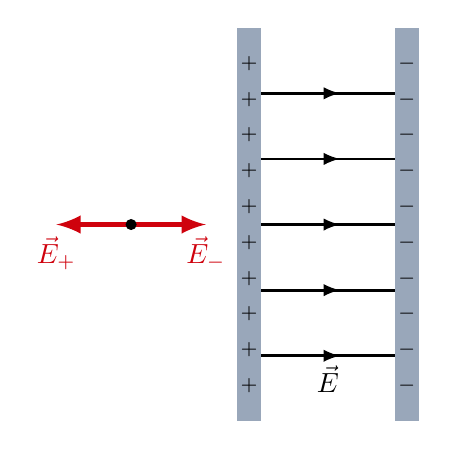
\begin{tikzpicture}
\tikzmath{
\L=2;
\h=5;
\nlines=5;
\dy=\h/(\nlines+1);
\platew=0.3;
}
\scalebox{1}{

\fill[color=myblue!40] (-\L/2-\platew/2,-\h/2) rectangle +(\platew,\h);
\fill[color=myblue!40] (\L/2-\platew/2,-\h/2) rectangle +(\platew,\h);

\foreach \i in{1,...,\nlines}{
  \draw[line width=1] (-\L/2+\platew/2, -\h/2+\i*\dy) -- +(\L-\platew,0);
  \draw[-latex, line width=1] (-\L/8, -\h/2+\i*\dy) -- +(0.2*\L,0);
  \ifthenelse{\i=1}{
   \node[below] at (0,-\h/2+\i*\dy) {$\vec E$};
  }
 }
 \foreach \i in{1,...,10}{
   \node[] at (-\L/2,-\h/2+\i*\h/11) {\scriptsize $+$};
   \node[] at (\L/2,-\h/2+\i*\h/11) {\scriptsize $-$};
 }
 \coordinate (P) at (-1.25*\L,0);
 \draw[latex-latex, line width=2,color=myred] ($(P)+(-0.95,0)$) node[below]{$\vec E_+$} -- ($(P)+(0.95,0)$) node[below]{$\vec E_-$};
 \fill (P) circle(2pt);

}
\end{tikzpicture}
\captionof*{figure}{\textit{Two oppositely-charged planes form a ``capacitor'', a device that can store energy.}}
\end{center}
}


%%%%%%%%%%%%%%%%%%%%%%%%%%%%%%%%
\subsection{Charges in and on a conductor}
\label{subsec:chargesinandonaconductor}
\twocolframesf{Charges in a conductor: Spherical shell}
{
\only<1>{
Consider a neutral spherical shell, when we place a charge $Q$ at its centre.
}
\only<2>{
\begin{itemize}
\item \textbf{The electric field inside of a conductor is always 0}, because the charges are free to move in a conductor.
\item If there is a field, charges will move until they have arranged themselves to not move anymore (this usually means that there is a separation of charge, leading to a net electric field of 0).
\end{itemize}
}
\only<3>{
We can use Gauss' Law to examine how charges are distributed inside conducting spherical shell with a charge $+Q$ placed at the centre:
\begin{itemize}
\item A negative charge, $-Q$, is induced on the inner surface of the conductor. There can be no flux through $S_1$ (thus no enclosed charge) because $S_1$ is inside a conductor, where the field must be zero.
\item A positive charge, $+Q$ is induced on the outer surface, since the shell is overall neutral.
\item The net charge enclosed by $S_2$ is:\\
 $(+Q) + (-Q) + (+Q) = +Q$ (as expected). 
\end{itemize}
Outside the spherical shell, the electric field is the same as it would be without the shell present!
}
}
{
\vspace{-0.5cm}
\begin{center}
\begin{tikzpicture}
\tikzmath{
\R1=1.5;
\R2=1.25*\R1;
\DelR=(\R2-\R1);
\Rmid=\R2-0.5*\DelR;
}
\scalebox{1}{

\only<2->{
\fill (0,0) circle(4pt) node[below=4pt]{$+Q$};
}
\shade[ball color=myblue!90, opacity=0.2] (0,0) circle(\R2);
\shade[ball color=myblue!10, opacity=0.3] (0,0) circle(\R1);

\only<2->{
\foreach \th in {0,30,...,330}{
  \node at (\th:\R1) {\scriptsize $-$};
  \node at (\th:1.0*\R2) {\scriptsize $+$};
}
}

\only<2>{
  \fill[color=myred] (45:\Rmid) circle(2pt);
  \draw[latex-latex, line width=1,color=myred] ($(45:\Rmid)+(45:0.75)$) node[above]{$\vec E_Q$} -- ($(45:\Rmid)+(45:-0.75)$) node[below]{$\vec E_{shell}$};
  \foreach \th in {0,10,...,350}{
  \draw[-latex,color=myred!50] (\th:\R2) -- (\th:\R1);
}

}

\only<3>{
 \draw[dotted, line width=2, color=myred] circle(1.05*\R1);
 \draw[dotted, line width=2, color=myred] circle(1.25*\R2);
 \node[color=myred] at (-90:0.85*\R1){$S_1$};
 \node[color=myred] at (-90:1.4*\R2){$S_2$};
 \node[left] at (90:0.7*\R1){$-Q$};
  \node[left] at (90:1.07*\R2){$+Q$};
}


}
\end{tikzpicture}
\captionof*{figure}{
\textit{\only<1>{A neutral metallic spherical shell.}\only<2>{Charges in a (neutral) conducting spherical shell will re-arrange themselves if a charge $+Q$ is placed at its centre (induction), leading to their own electric field.}\only<3>{Gauss' Law implies that the total charge induced on the inner and outer surfaces of the shell must have the same magnitude as the charge placed in the centre.}}}
\end{center}
%\capfig{0.4}{figures/chargesconductor}{Charges in a (neutral) conducting spherical shell will re-arrange themselves if a charge $+Q$ is placed at its centre (induction).}
}


%%%%%%%%%%%%%%%%%%%%%%%%%%%%%%%%
\twocolframesf{Charges \textit{on} a conductor}
{
There can be no charge inside a conductor.
Thus, if a conductor is charged, all the charges must be on the surface (otherwise, a closed surface in the conductor would enclose charge, thus have a net flux, thus have an electric field across the surface).

}
{
%\capfig{0.4}{figures/chargesconductor_pos}{On a charged conductor, charges must be on the surface.}
\vspace{-0.5cm}
\begin{center}
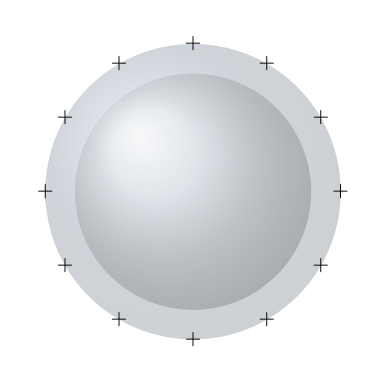
\begin{tikzpicture}
\tikzmath{
\R1=1.5;
\R2=1.25*\R1;
}
\scalebox{1}{

\shade[ball color=myblue!90, opacity=0.2] (0,0) circle(\R2);
\shade[ball color=myblue!10, opacity=0.3] (0,0) circle(\R1);

\foreach \th in {0,30,...,330}{
  \node at (\th:1.0*\R2) {\scriptsize $+$};
}

}
\end{tikzpicture}
\captionof*{figure}{\textit{On a charged conductor, such as a spherical shell, charges must be on the surface.}}
\end{center}
}

%%%%%%%%%%%%%%%%%%%%%%%%%%%%%



%%%%%%%%%%%%%%%%%%%%%%%%%%%%%%



%%%%%%%%%%%%%%%%%%%%%%%%%%%%



%%%%%%%%%%%%%%%%%%%%%%%%%%%%%
\end{document}





